%   File: PlanarParticleKinematics.tex
% Author: Adam Leeper
%------------------------------------------------------------------------------
%\\[0.45pc]
\providecommand{\isolatedBuild}[1]{#1}% fallback definition lets this file build normally
\isolatedBuild{
  \documentclass[11pt,letterpaper]{book}
  %\documentclass[11pt,letterpaper]{book}

% aleeper: I think these are needed for Paul's macros?
\usepackage{epsfig}
\usepackage{epstopdf}

%\makeatletter
%\typeout{The import path is \import@path}
%\makeatother

\usepackage{import}

\subimport{./}{packagesMitiguy.sty}
\subimport{./}{macrosMitiguy.tex}
\subimport{./}{PageStylesMitiguy.tex}
\subimport{./}{macrosLeeper.tex}
   % Must be found via TEXINPUTS environment variable.
  \isolatedBuildHeader{Planar Particle Kinematics}
                      {Planar Particle Kinematics - The Definitive Guide}
}
%%%
%%%
%%%
\section{Example: Deriving Kinematics Relationships for ``Circular" Motion}
%
\begin{minipage}[t]{0.70\linewidth}
  In this section we show clearly how to derive velocity and acceleration for a
  particle whose position is described by polar coordinates $r$ and $\theta$.
  In many ``traditional'' textbooks (Hibbeler, Beer and Johnson, \textit{etc}.)
  the mechanics of vector derivatives with rotating frames are not taught,
  so the kinematics expressions are simply given.
  However, deriving these quantities is a straight-forward
  application of the golden rule.
  %This is fine for a limited range of problems, but the equations can't be
  %used for complex 2D motion or nearly any 3D problems.
  % or those with mixedmost general situations, especially in 3-D (e.g. problem
  %7.11, 7.13) or with mixed motions (e.g. problem 7.9, 7.12, 7.14, 7.18 ).
  \\[0.45pc]
%
%  We always solve dynamics problems by forming:
%  \begin{itemize}
%    \item A description of the \textbf{motion}.
%    \item A description of the \textbf{mass}.
%    \item A description of the \textit{contact} and \textit{distance}
%          \textbf{forces}.
%  \end{itemize}
%  %\\[0.45pc]
%  \vspace{0.5pc}
%  Note that the first of these is \textbf{motion}. Specifically, we need an
%  expression for acceleration before we can do anything else.
%  %
%  \\[0.75pc]
  To ground the development with a concrete example, consider the figure
  shown at right. The disk is modeled as a rigid body
  \basis{B}, and its center $B_o$ is fixed in a Newtonian frame \basis{N}
  and co-incident with $N_o$. We define our usual \dextral, orthogonal unit
  vectors \uvecxyz{n} fixed in \basis{N} with \uvecx{n} horizontally right and
  \uvecy{n} vertically upward. Similarly, \uvecxyz{b} are fixed in \basis{B}
  with $\uvecz{b} = \uvecz{n}$ and \uvecx{b} pointing from $B_o$ to $Q$.
\end{minipage}
\hfill
\begin{minipage}[t]{0.25\linewidth}
  \vspace*{0pt}
  %\vspace*{-1.0pc}
  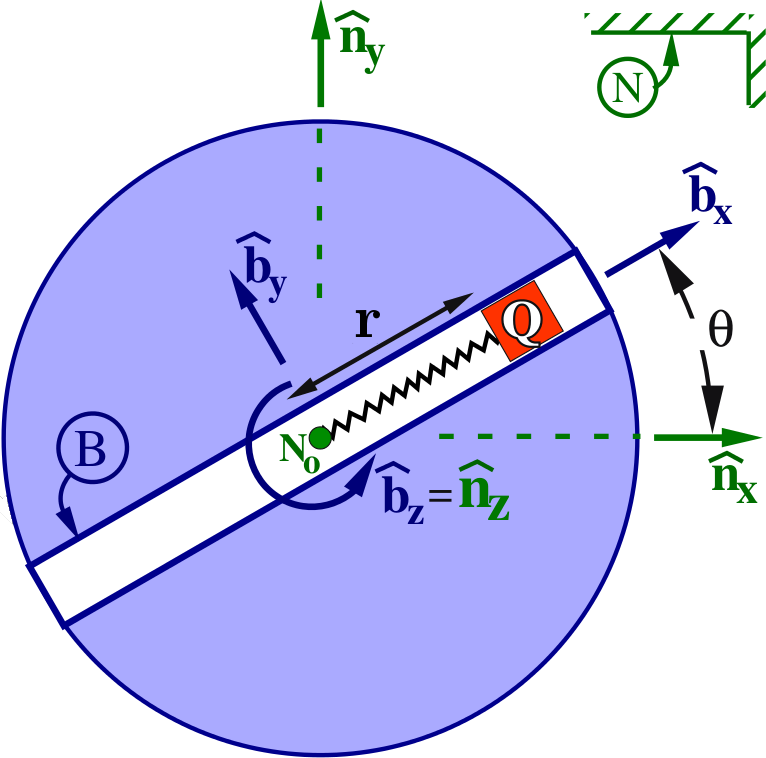
\includegraphics[width=1.0\linewidth]{disc_slot.png}
\end{minipage}
%
%
%
%
\vspace{-1.5pc}
\subsection{General Polar Kinematics}
We will differentiate the position vector to find velocity and acceleration
(note the ``two-points-fixed'' formulas don't apply because $Q$ is not fixed
on \basis{B}). We will need the angular velocity and angular
acceleration of \basis{B} in \basis{N}, which is formed \textbf{by inspection}
since \basis{B} has a \textbf{simple} rotation in \basis{N} about \uvecz{b}:
%\\[0.45pc]
$\angvel{B}{N} \equals[\;] \thetadot~\uvecz{b}$ and
$\alf{B}{N} \equals[\;] \thetaddot~\uvecz{b}$.
\\[0.45pc]
\textbf{Acceleration via Differentiation of Position Vector}
\\[0.45pc]
$\posvec{O}{P} \equals[] r~\uvecx{b}$
\\[0.45pc]
\begin{tabular}{@{}l@{~}c@{~}c@{~}c@{~}c l}
  %$\vel{P}{N} $\=$\deff[\hspace{0.2pc}] \dt[N]{}(\posvec{O}{P})$
  %\\[0.45pc]
  \vel{P}{N} & \deff & $ \dt[N]{}(~\posvec{O}{P}) $ & & &
  This is the \textbf{definition}.
\\[0.45pc]
           & \equals[\;] & $ \dt[N]{}(~r~\uvecx{b}) $   & & &
           So we \textbf{need} to differentiate this in \basis{N}.
\\[0.45pc]
           & \equals[\;] & $ \dt[B]{}(~r~\uvecx{b}) $ & $\plus[\;]$ &
           $\angvel{B}{N} \Cross (~r~\uvecx{b})$ &
           It's \textbf{easier} to differentiate this in \basis{B},
           so we use golden rule to convert.
\\[0.45pc]
           & \equals[\;] & $\rdot ~\uvecx{b}$ & $\plus[\;]$ &
           $ (\thetadot~\uvecz{b}) \Cross (~r~\uvecx{b})$ &
           \uvecx{b} is fixed in \basis{B}, so we can just
           differentiate the scalar portion.
\\[0.45pc]
   & \equals[\;] & $\rdot ~\uvecx{b}$ & \plus[\;] & $ r\thetadot~\uvecy{b}$ &
   And finally we do the cross product.
\end{tabular}
%
\\[1.0pc]
%
\begin{tabular}{@{}l@{~}c@{~}c@{~}c@{~}c@{~~}l}
  \accel{P}{N} & \deff & $ \dt[N]{}(~\vel{P}{N}) $ & & &
  This is the \textbf{definition}.
\\[0.45pc]
  & \equals[\;] & $ \dt[N]{}( ~\rdot ~\uvecx{b} \plus[\;]
  r\thetadot~\uvecy{b})$ & & &
  So we \textbf{need} to differentiate this in \basis{N}.
\\[0.45pc]
  & \equals[\;]  &$ \dt[B]{}(~\rdot ~\uvecx{b} \plus[\;] r\thetadot~\uvecy{b})$
  & $\plus[]$
  & $ \angvel{B}{N} \Cross (~\rdot ~\uvecx{b} \plus[\;] r\thetadot~\uvecy{b})$
  & \textbf{Easier} to differentiate in \basis{B}, so apply golden rule.
\\[0.45pc]
  & \equals[\;]
  & $ (~\rddot ~\uvecx{b} \plus[\;] (\rdot\thetadot + r \thetaddot)~\uvecy{b})$
  & $\plus[]$
  & $(\thetadot~\uvecz{b}) \Cross (~\rdot ~\uvecx{b} \plus[\;]
  r\thetadot~\uvecy{b})$
  & %\uvecx{b}, \uvecy{b} fixed in \basis{B},
    Differentiate scalars (remember \textbf{product rule}!).
\\[0.45pc]
  & \equals[\;]
  & $ (~\rddot ~\uvecx{b} \plus[\;] (\rdot\thetadot + r \thetaddot)~\uvecy{b})$
  & $\plus[]$
  & $(\rdot\thetadot~(\uvecy{b}) \plus[\;] r\thetadot^2~(-\uvecx{b}))$
  & Do cross product.
    %Note the duplicate $\rdot \thetadot ~\uvecy{b}$ term.
\\[0.45pc]
  & \equals[\;]
  & $ (~\rddot \minus[\;]  r\thetadot^2)~\uvecx{b}$
  & $\plus[]$
  & $(r\thetaddot \plus[\;] 2 \rdot \thetadot)~\uvecy{b}$
  & Collect terms.
\end{tabular}
\\[1.0pc]
Now that we have general expressions velocity and acceleration of a particle in planar motion expressed in polar coordinates, let's see how this can be specialized for some common scenarios.
%
%%%%%%%%%%%%%%%%%%%%%%%%%%%%%%%%%%%%%%%%%%%%%%%%%%%%%%%%%%%%%%%%%%%%%%%%%%%%%%%
%%%%%%%%%%%%%%%%%%%%%%%%%%%%%%%%%%%%%%%%%%%%%%%%%%%%%%%%%%%%%%%%%%%%%%%%%%%%%%%
%%%%%%%%%%%%%%%%%%%%%%%%%%%%%%%%%%%%%%%%%%%%%%%%%%%%%%%%%%%%%%%%%%%%%%%%%%%%%%%
%\clearpage
\subsection{Curvilinear Motion: Polar/Cylindrical Components}
Paraphrasing loosely, a ``traditional" book may say something like:
%
\begin{center}
  \fbox{
    \begin{minipage}{0.8\linewidth}
      ``For problems described by polar coordinates, you \textbf{must}
      assign a coordinate system with $\uveceR$ radially outward,
      $\uveceTheta$ perpendicular to $\uveceR$ and in the direction of
      increasing $\theta$,
      and $\uvecHat{e}_z = \uveceR \times \uveceTheta$.''
      (In our example, $\uveceR = \uvecx{b}$, $\uveceTheta = \uvecy{b}$,
      and $\uvecHat{e}_z = \uvecz{b}$.)
    \end{minipage}
  }
\end{center}
%
Then you would be given the following scalar values for the measures/components
of acceleration:
$$a_r \equals[\;] \rddot \minus[\;]  r\thetadot^2$$
$$a_\theta \equals[\;] r\thetaddot \plus[\;] 2 \rdot \thetadot$$
%$$a_z\equals[\;] \zdot$$

How do we get there from our expressions for \vel{Q}{N} and \accel{Q}{N}? In this class we get measures of a vector by dotting.
We can dot \accel{Q}{N} with ($\uveceR = \uvecx{b}$) ~and ($\uveceTheta = \uvecy{b}$) ~to get these same expressions:
\begin{center}
\begin{tabular}{l@{~}r@{~}c@{~}l}
   $a_r \equals[\;]$ & $\accel{Q}{N} \cdot \uveceR$ & \equals[\;] & $\rddot \minus[\;]  r\thetadot^2$
\\[0.45pc]
 $a_\theta \equals[\;]$ & $\accel{Q}{N} \cdot \uveceTheta$ & \equals[\;] & $r\thetaddot \plus[\;] 2 \rdot \thetadot$
\end{tabular}
\end{center}
It is \textbf{ok} to use these pre-computed expressions if you are
\textbf{sure} that you have the signs correct. However, it is often
convenient to assign frames in a different way (for example, in
problem 7.10 % (inverted pendulum on cart)
frame \basis{B} has $\uveceR = \uvecy{b}$ and $\uveceTheta = \uvecx{b}$ and in problem 7.9 and 7.16 % (helicopter retrieval, spring pendulum)
frame \basis{B} has $\uveceR = - \uvecy{b}$ and $\uveceTheta = \uvecx{b}$) so you cannot blindly use these expressions without accounting for this.
%
%\\[0.45pc]
%\textbf{(Differential) Equations of Motion:}
%\\[0.0pc]
%In a ``traditional" book you are told to use the following equations to form differential equations of motion:
%$$F_r      \equals[\;] m * a_r$$
%$$F_\theta \equals[\;] m * a_\theta$$
%%%$$F_z \equals[\;] m * a_z$$
%
%%Similar to before, this is simply the result of dotting the vector equation
%%$\force{Q} = m^Q * \accel{Q}{N}$ with \uveceR ~and \uveceTheta.
%So, how does this compare to what we have? If we use a free-body diagram to find the set of forces \force{Q} acting on $Q$, then we can write a \textbf{vector} equation that just so-happens to relate \accel{Q}{N} to \force{Q} using Newton's law.
%
%$$\force{Q} \equals[\;] m^Q * \accel{Q}{N}$$
%
%Now the ``dynamics'' is done and we just have a vector equation; if we want to solve for specific scalars we can dot with linearly independent unit vectors to get scalar equations.
%If we \textbf{choose} to dot with \uveceR ~and \uveceTheta,
%then our forces \force{Q} have been ``resolved" into force components $F_r$ that are in the \uveceR ~direction,
%and force components $F_\theta$ that are in the \uveceTheta ~direction. Similarly, the acceleration has been ``resolved" into components $a_r$ and $a_\theta$.
%%$$\force{Q} \equals[\;] m^Q * \accel{Q}{N}$$
%\begin{center}
%\begin{tabular}{ll@{~}c@{~}l}
%% & \force{Q} & \equals[\;] & $m^Q * \accel{Q}{N}$
%% \\[0.45pc]
%dot w/ \uveceR:     & $F_r$      & \equals[\;] & $m^Q * ~a_r$
%\\[0.45pc]
%dot w/ \uveceTheta: & $F_\theta$ & \equals[\;] & $m^Q * ~a_\theta$
%\end{tabular}
%\end{center}
%
%Note that we \textbf{do not have} to dot with \uveceR and \uveceTheta. There are times when it may be advantageous to dot with \uvecx{n}, \uvecy{n} instead; the resulting differential equations would look a bit different, but they would still be a valid description of the system dynamics. Hence, our approach of getting a vector equation first and \textbf{then choosing} which unit vectors to dot with is more powerful than simply being told ``here are the equations you use for polar coordinates."


%%%%%%%%%%%%%%%%%%%%%%%%%%%%%%%%%%%%%%%%%%%%%%%%%%%%%%%%%%%%%%%%%%%%%%%%%%%%%%%
%%%%%%%%%%%%%%%%%%%%%%%%%%%%%%%%%%%%%%%%%%%%%%%%%%%%%%%%%%%%%%%%%%%%%%%%%%%%%%%
%%%%%%%%%%%%%%%%%%%%%%%%%%%%%%%%%%%%%%%%%%%%%%%%%%%%%%%%%%%%%%%%%%%%%%%%%%%%%%%
%\clearpage
\subsection{Curvilinear Motion: Normal-Tangential Components}
Paraphrasing loosely, a ``traditional" book may say something like:
%
\begin{center}
  \fbox{
    \begin{minipage}{0.8\linewidth}
      ``When the path of a particle is \textbf{known}, it is possible to
      approximate its motion during a small interval as motion along a
      circular arc with radius $r$.
      You \textbf{must} assign a coordinate system with
      $\uvecuN$ radially \textbf{inward} and $\uvecuT$ tangent to the
      circular path in the direction of the particle's velocity."
      (In our example, $\uvecuN = -\uvecx{b}$ and $\uvecuT = \uvecy{b}$.)
    \end{minipage}
  }
\end{center}
%

Two implicit requirements of this model are that \textbf{during the short interval being considered}:
\begin{itemize}
\item the radius of the path is \textbf{constant} ($\rdot = \rddot = 0$).
\item the particle's velocity is purely tangential, described by a scalar $v$, where $v ~\deff~ \vel{Q}{N} \cdot \uvecuT$.
\end{itemize}
\vspace{0.5pc}
Then you would be given the following scalar values for the measures/components
of acceleration:
$$a_n \equals[\;] v^2 / r$$ % \frac{v^2}{r}$$
$$a_t \equals[\;] \vdot$$

How do we get there from our expressions for \vel{Q}{N} and \accel{Q}{N}?
If we plug in $\rdot = \rddot = 0$ we get:
$$ \vel{Q}{N} \equals[\;] ( 0 )~\uvecx{b} \plus[\;] (r\thetadot)~\uvecy{b}
              \equals[\;] r\thetadot~\uvecy{b} $$
$$ \accel{Q}{N} \equals[\;] ( 0 \minus[\;]  r\thetadot^2)~\uvecx{b}
                            \plus[\;] (r\thetaddot \plus[\;] 0)~\uvecy{b}
                \equals[\;] \minus[\;] r\thetadot^2~\uvecx{b}
                            \plus[\;] r\thetaddot~\uvecy{b} $$

Since we defined $v$ as the particle's tangential velocity measure, we can relate that to \vel{Q}{N} by dotting with the ``tangential" unit vector $\uvecuT = \uvecy{b}$,
and then also implicitly differentiating to get another relationship:
$$v ~\deff~ \vel{Q}{N} \cdot \uvecy{b}
\equals[\;] r \thetadot~\uvecy{b} \cdot \uvecy{b}
\equals[\;] r \thetadot$$
%
$$v \equals[\;] r \thetadot$$
$$\vdot \equals[\;] r \thetaddot$$

Hence we can re-write \vel{Q}{N} and \accel{Q}{N} by plugging in $\thetadot = v / r$ and $\thetaddot = \vdot / r$ to get:
$$ \vel{Q}{N} \equals[\;] v~\uvecy{b} $$
$$ \accel{Q}{N} \equals[\;] - (v^2/r)~\uvecx{b}
\plus[\;] \vdot~\uvecy{b} $$

Finally, to resolve acceleration into normal-tangential measures, we can dot with ($\uvecuN = - \uvecx{b}$) and ($\uvecuT = \uvecy{b}$).
\begin{center}
\begin{tabular}{r@{~}r@{~}c@{~}l}
   $a_n \equals[\;]$ & $\accel{Q}{N} \cdot \uvecuN$ &
   \equals[\;] & $v^2/r$
\\[0.45pc]
 $a_t \equals[\;]$ & $\accel{Q}{N} \cdot \uvecuT$ &
 \equals[\;] & $\vdot$
\end{tabular}
\end{center}
It is \textbf{ok} to use these pre-computed expressions if you are \textbf{sure} that you have the signs correct. However, it is often convenient to assign frames in a different way (for example, in
problem 7.7 % (roller coaster)
frame \basis{B} has $\uvecuN = -\uvecx{b}$ and $\uvecuT = \uvecy{b}$) so you cannot blindly use these expressions without accounting for this.
%
%\\[0.45pc]
%\textbf{(Differential) Equations of Motion:}
%\\[0.0pc]
%In a ``traditional" book you are told to use the following equations to form differential equations of motion:
%$$F_n \equals[\;] m * a_n$$
%$$F_t \equals[\;] m * a_t$$
%
%So, how does this compare to what we have? If we use a free-body diagram to find the set of forces \force{Q} acting on $Q$, then we can write a \textbf{vector} equation that just so-happens to relate \accel{Q}{N} to \force{Q} using Newton's law.
%
%$$\force{Q} \equals[\;] m^Q * \accel{Q}{N}$$
%
%Now the ``dynamics'' is done and we just have a vector equation; if we want to solve for specific scalars we can dot with linearly independent unit vectors to get scalar equations.
%If we \textbf{choose} to dot with \uvecuN ~and \uvecuT,
%then our forces have been ``resolved" into force components $F_n$ that are in the \uvecuN ~direction,
%and force components $F_t$ that are in the \uvecuT direction. Similarly, the acceleration has been ``resolved" into components $a_n$ and $a_t$.
%%$$\force{Q} \equals[\;] m^Q * \accel{Q}{N}$$
%\begin{center}
%\begin{tabular}{ll@{~}c@{~}l}
%% & \force{Q} & \equals[\;] & $m^Q * \accel{Q}{N}$
%% \\[0.45pc]
%dot w/ \uvecuN: & $F_n$ & \equals[\;] & $m^Q * ~a_n$
%\\[0.45pc]
%dot w/ \uvecuT: & $F_t$ & \equals[\;] & $m^Q * ~a_t$
%\end{tabular}
%\end{center}
%
%The last paragraph of the previous page also applies here.

%%%%%%%%%%%%%%%%%%%%%%%%%%%%%%%%%%%%%%%%%%%%%%%%%%%%%%%%%%%%%%%%%%%%%%%%%%%%%%%
%%%%%%%%%%%%%%%%%%%%%%%%%%%%%%%%%%%%%%%%%%%%%%%%%%%%%%%%%%%%%%%%%%%%%%%%%%%%%%%
%%%%%%%%%%%%%%%%%%%%%%%%%%%%%%%%%%%%%%%%%%%%%%%%%%%%%%%%%%%%%%%%%%%%%%%%%%%%%%%
%\clearpage
%\subsection*{Putting it together with forces}

%
%
%% ----------------------------------
%\clearpage
%
%\subsection*{Mass}
%The mass of $Q$ is simply described by the scalar $m^Q$. That was easy...
%
%\subsection*{Forces}
%Drawing a free-body-diagram on $Q$, we can \textbf{model} the contact and distance forces as follows:
%\begin{itemize}
%\item The disk exerts some contact force on $Q$. We can \textbf{choose} to express that contact force in terms of the unknown quantities $F_x~\uvecx{b} + F_y~\uvecy{b}$. This choice is not unique; it is just \textbf{one} way to express the contact force vector.
%\item The spring exerts a force $-k*x*\uvecx{b}$, since $x$ is measured as the extension from the natural length of the spring.
%\item We could include other forces, but we can argue that they would be very small and not significantly affect the equations.
%\end{itemize}
%Hence we get $\force{Q} = -k*x*\uvecx{b} + F_x~\uvecx{b} + F_y~\uvecy{b}$. Note we are assuming that the slot is ``smooth," which is an engineering keyword that should be screaming at you to say $F_x = 0$.
%
%\subsection*{Baking the Cake (or, putting the ingredients together)}
%We have some vectors, but they are of little use unless we can get some kind of equation in order to solve for unknowns, or to form differential equations. Fortunately, we can write a \textbf{vector} equation that just so-happens to relate \accel{Q}{N} to \force{Q} using Newton's law:
%$$\force{Q} \equals[\;] m^Q * \accel{Q}{N}$$
%$$-k*x*\uvecx{b} + F_y~\uvecy{b} \equals[\;]  (~\rddot \minus[\;]  r\thetadot^2)~\uvecx{b} \plus[\;] (r\thetaddot \plus[\;] 2 \rdot \thetadot)~\uvecy{b} $$
%
%We can do whatever we want with this vector equation; we can dot it with linearly independent unit vectors to get scalar equations.
%If we choose to dot with \uveceR ~and \uveceTheta,
%then our forces have been ``resolved" into force components $F_r$ that are in the \uveceR ~direction,
%and force components $F_\theta$ that are in the \uveceTheta direction. Similarly, the acceleration has been ``resolved" into components $a_r$ and $a_\theta$.
%\begin{center}
%\begin{tabular}{lr@{~}c@{~}l}
%dot w/ \uveceR:     & $F_r$      & \equals[\;] & $m * a_r$
%\\[0.45pc]
%dot w/ \uveceTheta: & $F_\theta$ & \equals[\;] & $m * a_\theta$
%\end{tabular}
%\end{center}
%

\isolatedBuildFooter
